
% \documentclass{standalone}
% \input{../tikz_header}

% \begin{document}

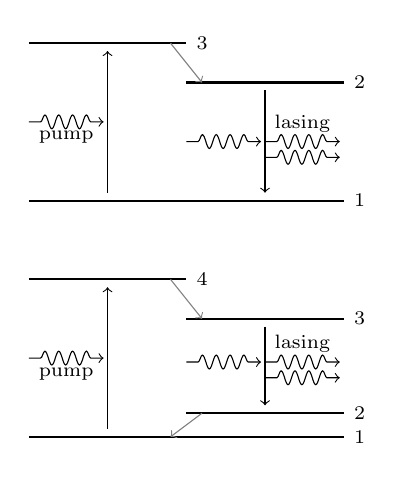
\begin{tikzpicture}[font=\scriptsize]
  
    \tikzstyle{photon}=[decorate,decoration={snake,pre length=0.15cm,post length=0.15cm,segment length=5}]



  \begin{scope}[yshift=+30mm]
    \draw[thick] (0,0) -- ++ (4,0) node[right] {1};
    \draw[thick] (0,2) -- ++ (2,0) node[right] {3};
    \draw[thick] (2,1.5) -- ++ (2,0) node[right] {2};

    \draw [->] (1,0.1) -- (1,1.9);
    \draw  [->, photon] (0, 1) -- node [below] {pump} +(+0.95,0);
    
    \draw [->, gray] (1.8,2) -- (2.2, 1.5);

    \draw [->] (3,1.4) -- (3,0.1);
    \draw  [->, photon] (2, 0.75) --  +(+0.95,0);
    \draw  [->, photon] (3, 0.75) -- node [above] {lasing}  +(+0.95,0);
    \draw  [->, photon] (3, 0.55) --  +(+0.95,0);
   \end{scope}

   \begin{scope}
    \draw[thick] (0,0) -- ++ (4,0) node[right] {1};
    \draw[thick] (0,2) -- ++ (2,0) node[right] {4};
    \draw[thick] (2,1.5) -- ++ (2,0) node[right] {3};
    \draw[thick] (2,0.3) -- ++ (2,0) node[right] {2};

    \draw [->] (1,0.1) -- (1,1.9);
    \draw  [->, photon] (0, 1) -- node [below] {pump} +(+0.95,0);
    
    \draw [->, gray] (1.8,2) -- (2.2, 1.5);

    \draw [->] (3,1.4) -- (3,0.4);
    \draw  [->, photon] (2, 0.95) --  +(+0.95,0);
    \draw  [->, photon] (3, 0.95) -- node [above] {lasing}  +(+0.95,0);
    \draw  [->, photon] (3, 0.75) --  +(+0.95,0);

    \draw [->, gray] (2.2,0.3) -- (1.8, 0);

   \end{scope}


\end{tikzpicture}

%\end{document}